El pedal de efectos tendrá una estructura clara: la parte más importante es la etapa de procesado, en la que se transforma la señal entrante en la que se va a proporcionar en la salida. La etapa de salida adquiere gran relevancia en sistemas que se diseñan para colacarse en cascada, ya que es importante adecuar la señal a los diferentes módulos. Pero en este capítulo se habla sobre la etapa de entrada. Esta etapa de entrada se encargará de captar la señal y prepararla para su procesado posterior por la FPGA.

\section{Selección de micrófono}

Para capturar el sonido, es necesario utilizar algún transductor que sea capaz de convertir la señal acústica consistente en ondas de presión en una serie de impulsos eléctricos. En el caso más común de instrumentos electrófonos, el uso de pedales es inmediato: la señal la viaja por un cable entre el instrumento y el amplificador, pero al enfocar este pedal a instrumentos de viento es necesaria esta conversión.

La solución más sencilla consiste en utilizar el micrófono que viene integrado con la placa Nexys A7: modelo \emph{ADMP421} de Analog Devices~\cite{Nexys}. No obstante, la utilización de este micrófono plantea dos problemas.

En primer lugar, es inmediato pensar que incluso en el caso de un prototipo, si se plantea usar como pedal, no resulta nada recomendable colocar el micrófono encargado de recoger todo el sonido en el suelo. Además de estar lejos de la fuente sonora, capturaría el sonido resultante de la manipulación de los controles suponiendo una bajada en la calidad del sonido que pudiese proporcionar el dispositivo.

\begin{figure}
\begin{center}
\label{fig:polar_dig}
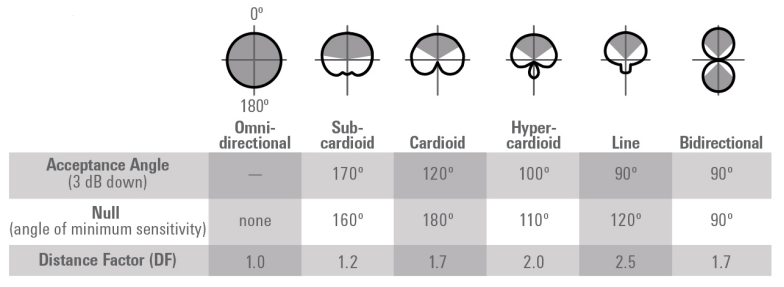
\includegraphics[width=15cm]{img/micros.png}
\caption{Tipos de micrófonos según su diagrama polar~\cite{Mic}}
\end{center}
\end{figure}

En segundo lugar, pero no menos importante, conviene tener en cuenta la respuesta de sensibilidad del micrófono será omnidireccional, es decir, captará todos los sonidos sin importar la dirección de dónde vengan. Este tipo de aparatos se usa principalmente en radio y televisión, donde puede haber varias personas hablando en el mismo micrófono o para la grabación de orquestas o agrupaciones en localizaciones cerradas determinadas. Estos micrófonos son capaces de captar tanto el sonido proveniente de la fuente directamente como los ecos y reflexiones característicos del espacio, dando la sensación de amplitud al oyente que la que produciría su escucha en esa misma localización. Pero mientras que en estos casos se trata de un efecto deseado, resulta poco agradable captar estas reflexiones en un ambiente no preparado para ello y en general, se suelen utilizar micrófonos de tipo cardioide.

Estos micrófonos son muy utilizados con instrumentos de viento, ya que el sonido suele provenir de un punto concreto. Es preciso matizar que en el caso del saxofón, contra la creencia popular, el sonido no sale siempre por la campana del instrumento. El sonido sale, por el contrario, por la llave abierta más cercana a la embocadura, que suele ser en torno al centro del instrumento. Por lo que tampoco resulta conveniente acercar el micrófono mucho a la campana dado que se descuidan las otras llaves del instrumento. La figura \ref{fig:saxo} muestra un saxofón en detalle.

\begin{figure}[!b]
\begin{center}
\label{fig:saxo}
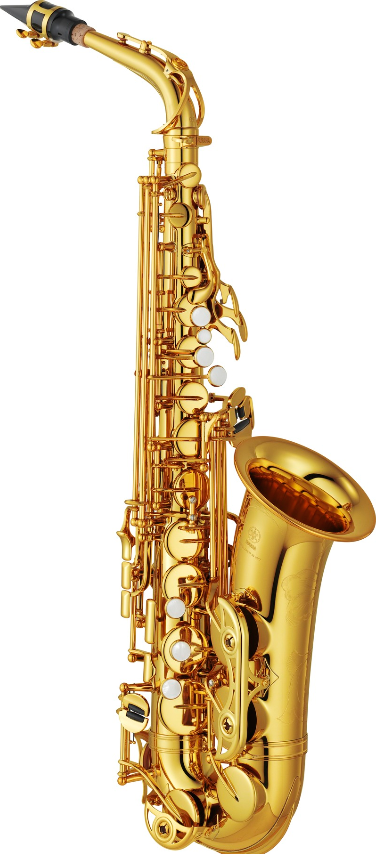
\includegraphics[height=9cm]{img/saxo.png}
\caption{Saxofón alto}
\end{center}
\end{figure}
